\documentclass[12pt]{article}
\usepackage[utf8]{inputenc}
\usepackage[utf8]{inputenc}
\usepackage{amsmath}
\usepackage{amsthm}
\usepackage{amssymb}
\usepackage{geometry}
\usepackage{amsfonts}
\usepackage{mathrsfs}
\usepackage{bm}
\usepackage{hyperref}
\usepackage[dvipsnames]{xcolor}
\usepackage[inline]{enumitem}
\usepackage{mathtools}
\usepackage{changepage}
\usepackage{graphicx}
\usepackage{caption}
\usepackage{subcaption}
\usepackage{lipsum}
\usepackage{tikz}
\usetikzlibrary{matrix, patterns, decorations.pathreplacing, calligraphy}
\usepackage{tikz-cd}
\usepackage[nameinlink]{cleveref}
\geometry{
headheight=15pt,
left=60pt,
right=60pt
}
\setlength{\emergencystretch}{20pt}
\usepackage{fancyhdr}
\pagestyle{fancy}
\fancyhf{}
\lhead{}
\chead{Section 5.4 Exercises}
\rhead{\thepage}
\hypersetup{
    colorlinks=true,
    linkcolor=blue,
    urlcolor=blue
}

\theoremstyle{definition}
\newtheorem*{remark}{Remark}

\newtheoremstyle{exercise}
    {}
    {}
    {}
    {}
    {\bfseries}
    {.}
    { }
    {\thmname{#1}\thmnumber{#2}\thmnote{ (#3)}}
\theoremstyle{exercise}
\newtheorem{exercise}{Exercise 5.4.}

\newtheoremstyle{solution}
    {}
    {}
    {}
    {}
    {\itshape\color{magenta}}
    {.}
    { }
    {\thmname{#1}\thmnote{ #3}}
\theoremstyle{solution}
\newtheorem*{solution}{Solution}

\Crefformat{exercise}{#2Exercise 5.4.#1#3}

\newcommand{\interior}[1]{%
  {\kern0pt#1}^{\mathrm{o}}%
}
\newcommand{\ts}{\textsuperscript}
\newcommand{\setcomp}[1]{#1^{\mathsf{c}}}
\newcommand{\quand}{\quad \text{and} \quad}
\newcommand{\N}{\mathbf{N}}
\newcommand{\Z}{\mathbf{Z}}
\newcommand{\Q}{\mathbf{Q}}
\newcommand{\I}{\mathbf{I}}
\newcommand{\R}{\mathbf{R}}
\newcommand{\C}{\mathbf{C}}

\DeclarePairedDelimiter\abs{\lvert}{\rvert}
% Swap the definition of \abs* and \norm*, so that \abs
% and \norm resizes the size of the brackets, and the 
% starred version does not.
\makeatletter
\let\oldabs\abs
\def\abs{\@ifstar{\oldabs}{\oldabs*}}
%
\let\oldnorm\norm
\def\norm{\@ifstar{\oldnorm}{\oldnorm*}}
\makeatother

\DeclarePairedDelimiter\paren{(}{)}
\makeatletter
\let\oldparen\paren
\def\paren{\@ifstar{\oldparen}{\oldparen*}}
\makeatother

\DeclarePairedDelimiter\bkt{[}{]}
\makeatletter
\let\oldbkt\bkt
\def\bkt{\@ifstar{\oldbkt}{\oldbkt*}}
\makeatother

\DeclarePairedDelimiter\set{\{}{\}}
\makeatletter
\let\oldset\set
\def\set{\@ifstar{\oldset}{\oldset*}}
\makeatother

\setlist[enumerate,1]{label={(\alph*)}}

\begin{document}

\section{Section 5.4 Exercises}

Exercises with solutions from Section 5.4 of \hyperlink{ua}{[UA]}.

\begin{exercise}
\label{ex:1}
    Sketch a graph of \( (1/2)h(2x) \) on \( [-2, 3] \). Give a qualitative description of the functions
    \[
        h_n(x) = \frac{1}{2^n} h(2^n x)
    \]
    as \( n \) gets larger.
\end{exercise}

\begin{solution}
    See \Cref{fig:1} for the sketch.
    \begin{figure}[ht]
        \centering
        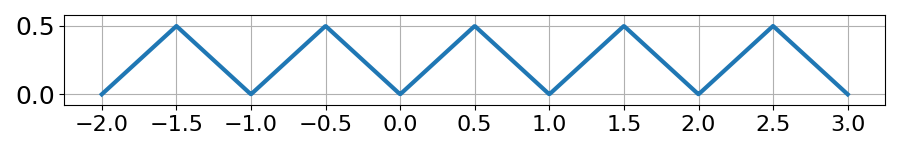
\includegraphics[width=14cm]{UA_Section_5_4_Figure_1.png}
        \caption{\( (1/2) h(2x) \)}
        \label{fig:1}
    \end{figure}
    Each \( h_n \) is a periodic ``sawtooth'' function; as \( n \) gets larger, the ``teeth'' get more densely packed and the peaks get lower.
\end{solution}

\begin{exercise}
\label{ex:2}
    Fix \( x \in \R \). Argue that the series
    \[
        \sum_{n=0}^{\infty} \frac{1}{2^n} h(2^n x)
    \]
    converges and thus \( g(x) \) is properly defined.
\end{exercise}

\begin{solution}
    Note that for each \( n \in \N \) we have \( 0 \leq 2^{-n} h(2^n x) \leq 2^{-n} \) since \( 0 \leq h(x) \leq 1 \). As the series \( \sum_{n=0}^{\infty} 2^{-n} \) is convergent (Example 2.7.5), the series \( \sum_{n=0}^{\infty} 2^{-n} h(2^n x) \) is also convergent by the Comparison Test (Theorem 2.7.4).
\end{solution}

\begin{exercise}
\label{ex:3}
    Taking the continuity of \( h(x) \) as given, reference the proper theorems from Chapter 4 that imply that the \textit{finite} sum
    \[
        g_m(x) = \sum_{n=0}^m \frac{1}{2^n} h(2^n x)
    \]
    is continuous on \( \R \).
\end{exercise}

\begin{solution}
    The continuity of \( g_m \) follows from Theorem 4.3.4 and Theorem 4.3.9.
\end{solution}

\begin{exercise}
\label{ex:4}
    As the graph of Figure 5.7 suggests, the structure of \( g(x) \) is quite intricate. Answer the following questions, assuming that \( g(x) \) is indeed continuous.
    \begin{enumerate}
        \item How do we know \( g \) attains a maximum value \( M \) on \( [0, 2] \)? What is this value?

        \item Let \( D \) be the set of points in \( [0, 2] \) where \( g \) attains its maximum. That is \( D = \{ x \in [0, 2] : g(x) = M \} \). Find one point in \( D \).

        \item Is \( D \) finite, countable, or uncountable?
    \end{enumerate}
\end{exercise}

\begin{solution}
    \begin{enumerate}
        \item Since \( g \) is continuous on the compact set \( [0, 2] \), we know it attains a maximum here by the Extreme Value Theorem (Theorem 4.4.2). To find this maximum value \( M \), for each non-negative integer \( n \) let \( f_n(x) = 2^{-2n} h(2^{2n} x) + 2^{-2n - 1} h(2^{2n+1} x) \), so that
        \[
            f_0(x) = h(x) + \frac{1}{2} h(2 x), \quad f_1(x) = \frac{1}{4} h(4 x) + \frac{1}{8} h(8 x), \quad \text{etc}.
        \]
        Thus
        \[
            g(x) = h(x) + \frac{1}{2} h(2 x) + \frac{1}{4} h(4 x) + \frac{1}{8} h(8 x) + \cdots = f_0(x) + f_1(x) + \cdots.
        \]
        (For any given \( x \), such a regrouping of terms is justified since we showed in \Cref{ex:2} that the series defining \( g(x) \) is convergent; see \href{https://lew98.github.io/Mathematics/UA_Section_2_5_Exercises.pdf}{Exercise 2.5.3}.)

        See \Cref{fig:1sub1} for a graph of \( f_0 \) on \( [0, 2] \) and note that \( f_0(x) = 1 \) on the interval \( \bkt{\tfrac{1}{2}, \tfrac{3}{2}} \). Furthermore, observe that \( f_1(x) = \tfrac{1}{4} f_0(4x) \), so that on the interval \( [0, 2] \) the function \( f_1 \) is given by four copies of \( f_0 \) scaled by a factor of \( \tfrac{1}{4} \). The interval \( \bkt{\tfrac{1}{2}, \tfrac{3}{2}} \), where \( f_0 \) is constant, contains two of the intervals of length \( \tfrac{1}{4} \) where \( f_1 \) is also constant; see \Cref{fig:1sub2}. On these intervals, we then have \( f_0(x) + f_1(x) = 1 + \tfrac{1}{4} \). Similarly, \( f_2 \) is given by \( f_2(x) = \tfrac{1}{16} f_0(16x) \). Furthermore, there are further subintervals of the previous subintervals where \( f_2 \) is also constant and thus, on these subintervals, we have \( f_0(x) + f_1(x) + f_2(x) = 1 + \tfrac{1}{4} + \tfrac{1}{16} \); see \Cref{fig:1sub3}.

        We can continue arguing in this manner to see that \( M \geq 1 + \tfrac{1}{4} + \tfrac{1}{16} + \cdots = \tfrac{4}{3} \). On the other hand, since each \( f_n \) satisfies \( f_n(x) \leq 4^{-n} \) on \( [0, 2] \), we have
        \[
            g(x) = f_0(x) + f_1(x) + f_2(x) + \cdots \leq 1 + \frac{1}{4} + \frac{1}{16} + \cdots = \frac{4}{3}.
        \]
        We may conclude that \( M = \tfrac{4}{3} \).

        \begin{figure}
            \centering
            \begin{subfigure}{0.49\textwidth}
              \centering
              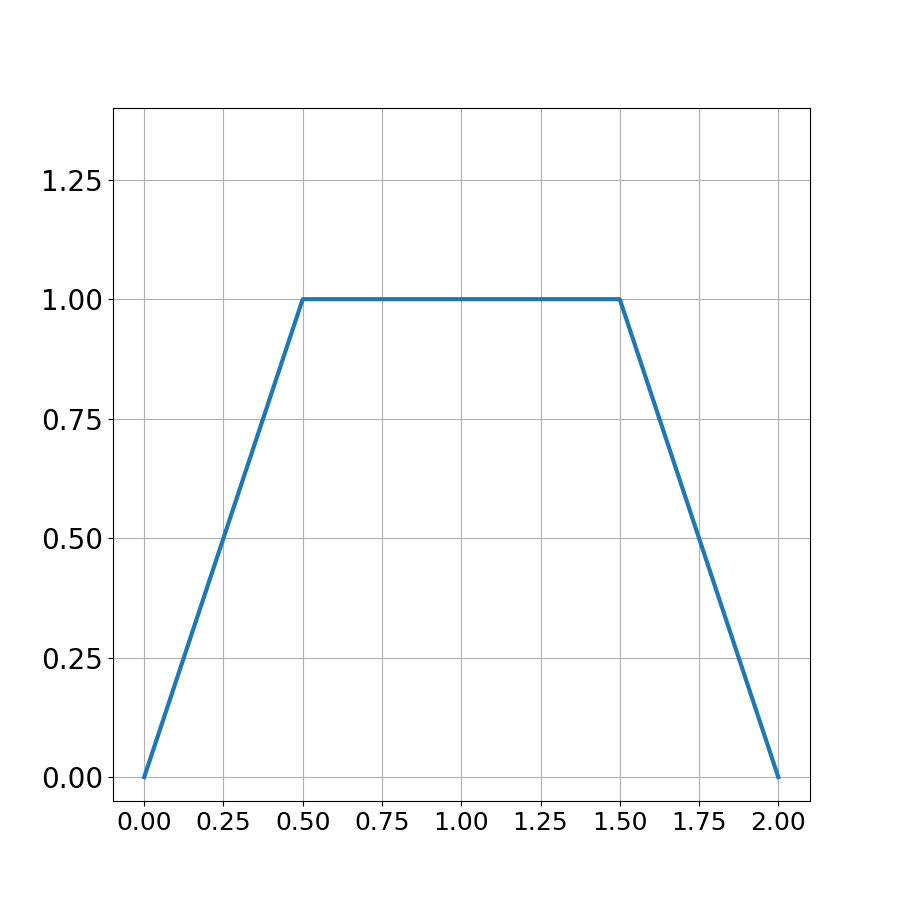
\includegraphics[width=\linewidth]{UA_Section_5_4_Figure_2.png}
              \caption{\( f_0(x) \) on \( [0, 2] \)}
              \label{fig:1sub1}
            \end{subfigure}%
            \begin{subfigure}{0.49\textwidth}
              \centering
              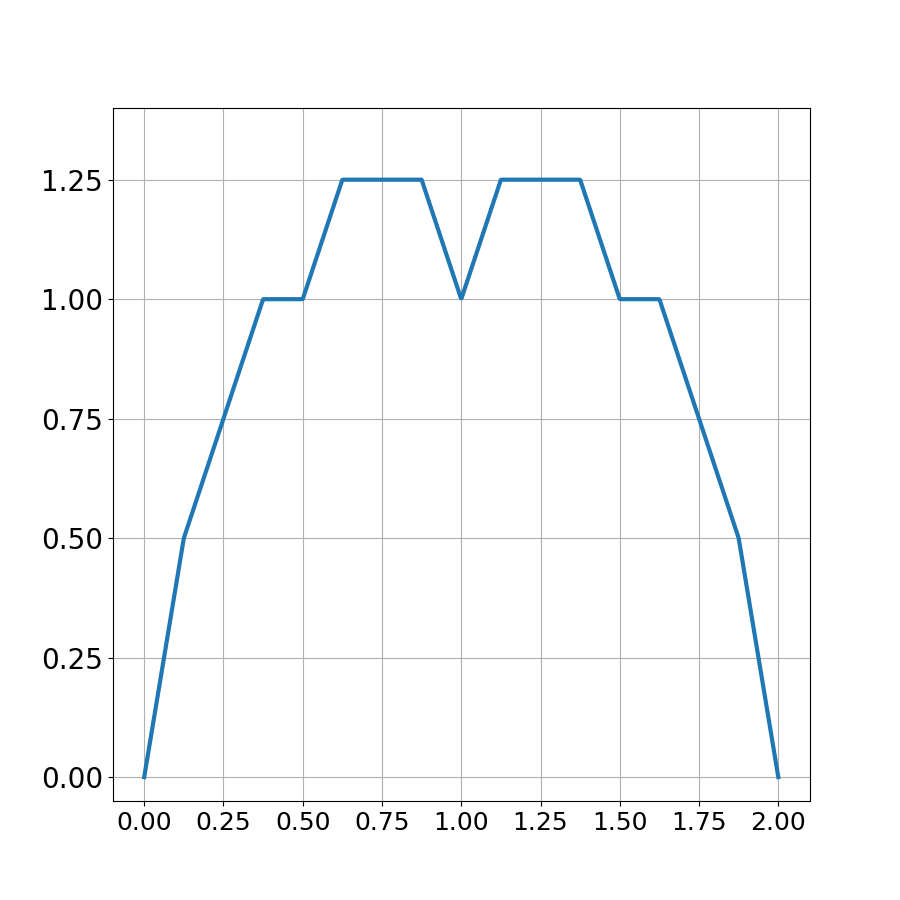
\includegraphics[width=\linewidth]{UA_Section_5_4_Figure_3.png}
              \caption{\( f_0(x) + f_1(x) \) on \( [0, 2] \)}
              \label{fig:1sub2}
            \end{subfigure}

            \begin{subfigure}{0.5\textwidth}
                \centering
                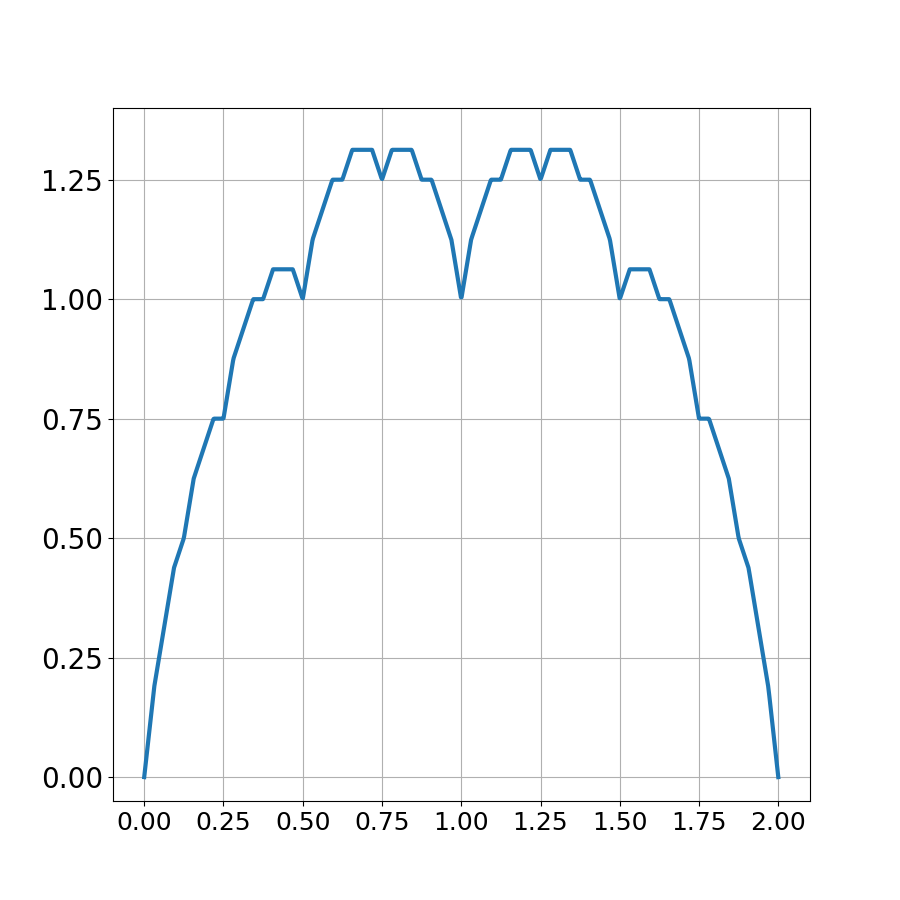
\includegraphics[width=\linewidth]{UA_Section_5_4_Figure_4.png}
                \caption{\( f_0(x) + f_1(x) + f_2(x) \) on \( [0, 2] \)}
                \label{fig:1sub3}
              \end{subfigure}
            \caption{Function graphs for \Cref{ex:4}}

            \label{fig:2}
        \end{figure}

        \item Let us show that for every non-negative integer \( n \), we have \( h \paren{\tfrac{2^{n+1}}{3}} = \tfrac{2}{3} \). The base case \( n = 0 \) is clear. Suppose that the result is true for some \( n \). Observe that
        \[
            h \paren{\tfrac{2^{n+2}}{3}} = h \paren{\tfrac{2^{n+2}}{3} - 2^{n+1}} = h \paren{\tfrac{2^{n+1}(2 - 3)}{3}} = h \paren{-\tfrac{2^{n+1}}{3}} = h \paren{\tfrac{2^{n+1}}{3}} = \frac{2}{3},
        \]
        where we have used our induction hypothesis and the fact that \( h \) is an even 2-periodic function. It follows by induction that \( h \paren{\tfrac{2^{n+1}}{3}} = \tfrac{2}{3} \) for all non-negative integers \( n \).

        Now observe that
        \[
            g \paren{\tfrac{2}{3}} = \sum_{n=0}^{\infty} \frac{1}{2^n} h \paren{\tfrac{2^{n+1}}{3}} = \frac{2}{3} \sum_{n=0}^{\infty} \frac{1}{2^n} = \frac{4}{3} = M.
        \]
        Thus \( \tfrac{2}{3} \in D \).

        \item We will show that \( D \) is uncountable. In fact, we will prove a stronger statement: \( D \) is in bijection with \( \R \). To do this, we will inject a space of binary sequences into \( D \); after appealing to results we proved in Section 1.5 and Section 1.6, this will allow us to conclude the desired result.

        \begin{figure}
            \centering
            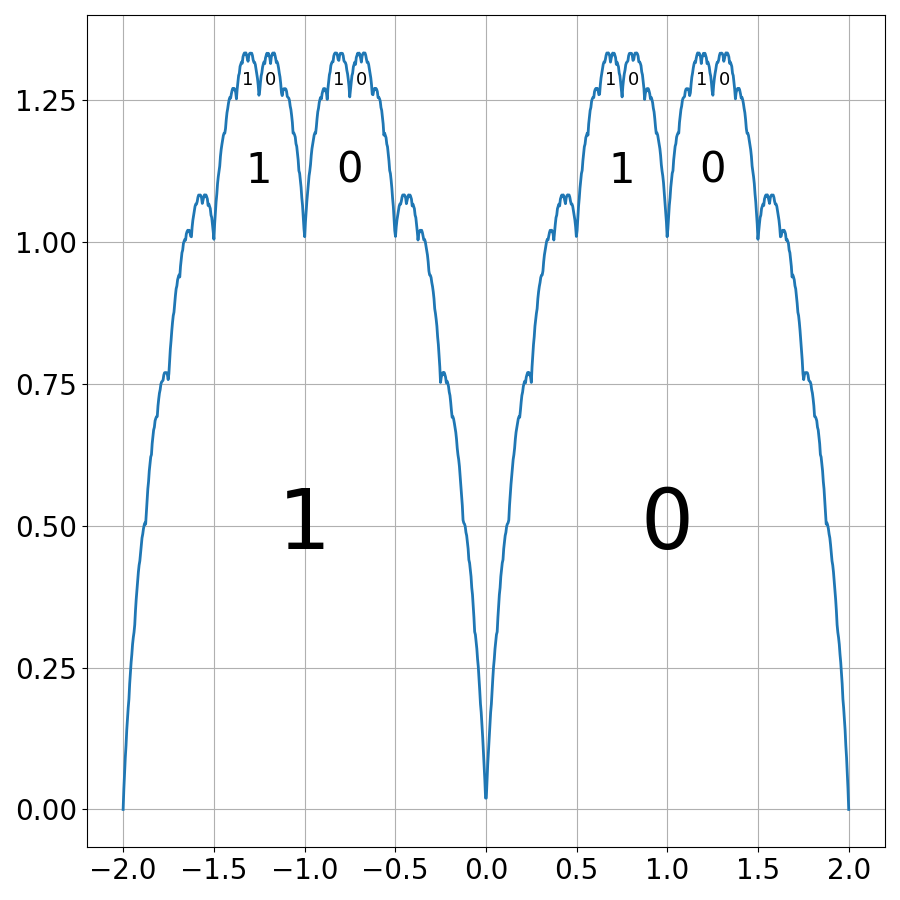
\includegraphics[width=16cm]{UA_Section_5_4_Figure_5.png}
            \caption{\( g \) on \( [-2, 2] \)}
            \label{fig:3}
        \end{figure}
        
        First, suppose that \( b : \{ 0, 1, 2, \ldots \} \to \{ 0, 1 \} \) satisfies \( b(0) = 0 \). We claim that
        \[
            x_b := \sum_{k=0}^{\infty} \frac{(-1)^{b(k)}}{4^k} = 1 + \sum_{k=1}^{\infty} \frac{(-1)^{b(k)}}{4^k}
        \]
        belongs to \( D \), i.e.\ satisfies \( x_b \in [0, 2] \) and \( g(x_b) = M = \tfrac{4}{3} \). (For the intuition here, see \Cref{fig:3}. The choice of \( b(0) = 0 \) guarantees that \( x_b \in [0, 2] \); a choice of \( b(0) = 1 \) would give us \( x_b \in [-2 , 0] \).) To see this, observe that
        \[
            x_b \leq \sum_{k=0}^{\infty} \frac{1}{4^k} = \frac{4}{3} \quand x_b \geq 1 - \sum_{k=1}^{\infty} \frac{1}{4^k} = \frac{2}{3}
        \]
        and thus \( x_b \in [0, 2] \). Now let us express \( g \) as
        \[
            g(x) = \sum_{n=0}^{\infty} \frac{1}{4^n} f_0(4^n x). 
        \]
        (See part (a) for the definition of \( f_0 \) and the justification for this expression; also see \Cref{fig:1sub1} for a graph of \( f_0 \) on the interval \( [0, 2] \).) Suppose that \( K \) is a non-negative integer and \( n \geq K + 1 \). Observe that
        \[
            4^n \paren{1 + \frac{(-1)^{b(1)}}{4} + \cdots + \frac{(-1)^{b(K)}}{4^K} }
        \]
        is an even integer and thus by the 2-periodicity of \( f_0 \) we have
        \[
            f_0 \paren{ 4^n \paren{1 + \frac{(-1)^{b(1)}}{4} + \cdots + \frac{(-1)^{b(K)}}{4^K} } } = f_0(0) = 0.
        \]
        Furthermore, observe that
        \[
            4^K \paren{1 + \frac{(-1)^{b(1)}}{4} + \cdots + \frac{(-1)^{b(K)}}{4^K} }
        \]
        is an odd integer and thus by the 2-periodicity of \( f_0 \) we have
        \[
            f_0 \paren{ 4^K \paren{1 + \frac{(-1)^{b(1)}}{4} + \cdots + \frac{(-1)^{b(K)}}{4^K} } } = f_0(1) = 1.
        \]
        Now, if \( K \geq 1 \), suppose that \( 0 \leq n \leq K - 1 \). Then
        \begin{multline*}
            4^n \paren{1 + \frac{(-1)^{b(1)}}{4} + \cdots + \frac{(-1)^{b(K)}}{4^K} } \\ = \underbrace{4^n + (-1)^{b(1)} 4^{n-1} + \cdots + (-1)^{b(n)}}_{\text{odd integer}} + \frac{(-1)^{b(n+1)}}{4} + \cdots + \frac{(-1)^{b(k)}}{4^{K-n}}.
        \end{multline*}
        It follows from the 2-periodicity of \( f_0 \) that
        \[
            f_0 \paren{ 4^n \paren{1 + \frac{(-1)^{b(1)}}{4} + \cdots + \frac{(-1)^{b(K)}}{4^K} } } = f_0 \paren{ 1 + \frac{(-1)^{b(n+1)}}{4} + \cdots + \frac{(-1)^{b(k)}}{4^{K-n}} }.
        \]
        Note that
        \[
            \frac{2}{3} = 1 - \sum_{k=0}^{\infty} \frac{1}{4^k} \leq 1 + \frac{(-1)^{b(n+1)}}{4} + \cdots + \frac{(-1)^{b(k)}}{4^{K-n}} \leq \sum_{k=0}^{\infty} \frac{1}{4^k} = \frac{4}{3}.
        \]
        Since \( f_0(x) = 1 \) on the interval \( \bkt{\tfrac{2}{3}, \tfrac{4}{3}} \), we see that
        \[
            f_0 \paren{ 1 + \frac{(-1)^{b(n+1)}}{4} + \cdots + \frac{(-1)^{b(k)}}{4^{K-n}} } = 1.
        \]
        To summarize our findings, for each non-negative integer \( K \) we have
        \[
            f_0 \paren{ 4^n \sum_{k=0}^K \frac{(-1)^{b(k)}}{4^k} } = \begin{cases}
                1 & \text{if } 0 \leq n \leq K, \\
                0 & \text{if } n > K.
            \end{cases}
            \tag{1}
        \]
        We can now show that \( g(x_b) = \tfrac{4}{3} \):
        \begin{align*}
            g(x_b) &= g \paren{ \lim_{K \to \infty} \sum_{k=0}^K \frac{(-1)^{b(k)}}{4^k} } \\[2mm]
            &= \lim_{K \to \infty} g \paren{ \sum_{k=0}^K \frac{(-1)^{b(k)}}{4^k} } \tag{since \( g \) is continuous} \\[2mm]
            &= \lim_{K \to \infty} \sum_{n=0}^{\infty} \frac{1}{4^n} f_0 \paren{4^n \sum_{k=0}^K \frac{(-1)^{b(k)}}{4^k}} \\[2mm]
            &= \lim_{K \to \infty} \sum_{n=0}^K \frac{1}{4^n} \tag{by (1)} \\[2mm]
            &= \sum_{n=0}^{\infty} \frac{1}{4^n} \\[2mm]
            &= \frac{4}{3}.
        \end{align*}
        If we let \( B \) be the following space of binary sequences
        \[
            B := \{ b : \{ 0, 1, 2, \ldots \} \to \{ 0, 1 \} \text{ such that } b(0) = 0 \},
        \]
        and define a function \( \Psi : B \to D \) by \( \Psi(b) = x_b \), we have now shown that \( \Psi \) is well-defined and maps into \( D \). Our next claim is that \( \Psi \) is injective. To see this, suppose that \( a, b \in B \) and \( a \neq b \). Let
        \[
            K := \min \{ k \geq 0 : a(k) \neq b(k) \};
        \]
        without loss of generality, we may assume that \( a(K) = 1 \) and \( b(K) = 0 \). Thus
        \begin{gather*}
            x_a = 1 + \frac{(-1)^{a(1)}}{4} + \frac{(-1)^{a(2)}}{16} + \cdots - \frac{1}{4^K} + \frac{(-1)^{a(K+1)}}{4^{K+1}} + \cdots, \\[2mm]
            x_b = 1 + \frac{(-1)^{a(1)}}{4} + \frac{(-1)^{a(2)}}{16} + \cdots + \frac{1}{4^K} + \frac{(-1)^{b(K+1)}}{4^{K+1}} + \cdots.
        \end{gather*}
        It follows that
        \[
            x_b - x_a = \frac{2}{4^K} + \frac{(-1)^{b(K+1)} - (-1)^{a(K+1)}}{4^{K+1}} + \frac{(-1)^{b(K+2)} - (-1)^{a(K+2)}}{4^{K+2}} + \cdots
        \]
        and hence that
        \begin{align*}
            4^{-K}(x_b - x_a) - 2 &= \frac{(-1)^{b(K+1)} - (-1)^{a(K+1)}}{4} + \frac{(-1)^{b(K+2)} - (-1)^{a(K+2)}}{16} + \cdots \\[2mm]
            &\geq -2 \paren{ \frac{1}{4} + \frac{1}{16} + \cdots } \\[2mm]
            &= -\frac{2}{3}.
        \end{align*}
        Thus \( 4^{-K} (x_b - x_a) \geq \frac{4}{3} > 0 \), which implies that \( x_b > x_a \) and hence \( \Psi \) is injective.

        It is straightforward to show that the map \( B \to P(\N) \), where \( P(\N) \) is the power set of \( \N \), given by
        \[
            b \mapsto \{ n \in \N : b(n) = 1 \}
        \]
        has an inverse given by
        \[
            A \subseteq \N \mapsto \paren{ n \mapsto \begin{cases}
                1 & \text{if } n \in A, \\
                0 & \text{if } n \not\in A,
            \end{cases}
            } 
        \]
        so that \( B \) is in bijection with \( P(\N) \). As we showed in \href{https://lew98.github.io/Mathematics/UA_Section_1_6_Exercises.pdf}{Exercise 1.6.9}, \( P(\N) \) is in bijection with \( \R \). The inclusion \( D \hookrightarrow \R \) thus provides us with an injection \( D \to B \). The Schröder-Bernstein Theorem (see \href{https://lew98.github.io/Mathematics/UA_Section_1_5_Exercises.pdf}{Exercise 1.5.11}) allows us to conclude that \( D \) is in bijection with \( \R \) and hence is uncountable.
    \end{enumerate}
\end{solution}

\begin{exercise}
\label{ex:5}
    Show that
    \[
        \frac{g(x_m) - g(0)}{x_m - 0} = m + 1,
    \]
    and use this to prove that \( g'(0) \) does not exist.
\end{exercise}

\begin{solution}
    For any \( m \in \{ 0, 1, 2, \ldots \} \), we have
    \[
        h(2^{n - m}) = \begin{cases}
            2^{n - m} & \text{if } 0 \leq n \leq m, \\
            0 & \text{if } n > m.
        \end{cases}
    \]
    (In the \( 0 \leq n \leq m \) case we have \( 0 < 2^{n - m} \leq 1 \) and in the \( n > m \) case we have that \( 2^{n - m} \) is an even integer; the 2-periodicity of \( h \) then implies that \( h(2^{n - m}) = h(0) = 0 \).) Thus
    \[
        g(x_m) = \sum_{n=0}^{\infty} \frac{1}{2^n} h(2^{n - m}) = \sum_{n=0}^m \frac{1}{2^m} = \frac{m + 1}{2^m},
    \]
    which gives us
    \[
        \frac{g(x_m) - g(0)}{x_m} = 2^m g(x_m) = m + 1.
    \]
    Since \( \lim_{m \to \infty} x_m = 0 \) and
    \[
        \lim_{m \to \infty} \frac{g(x_m)}{x_m} = \lim_{m \to \infty} m + 1 = +\infty,
    \]
    it follows that the limit \( \lim_{x \to 0} \frac{g(x)}{x} \) does not exist, i.e.\ \( g'(0) \) does not exist.
\end{solution}

\begin{exercise}
\label{ex:6}
    \begin{enumerate}
        \item Modify the previous argument to show that \( g'(1) \) does not exist. Show that \( g'(1/2) \) does not exist.

        \item Show that \( g'(x) \) does not exist for any rational number of the form \( x = p/2^k \) where \( p \in \Z \) and \( k \in \N \cup \{ 0 \} \).
    \end{enumerate}
\end{exercise}

\begin{solution}
    \begin{enumerate}
        \item These are both special cases of the result in part (b); for the sake of brevity, we omit these proofs.

        \item Let \( (x_m) \) be the sequence defined by \( x_m = x + 2^{-m} = p 2^{-k} + 2^{-m} \). Since we are interested in the limiting behaviour as \( m \to \infty \), we may assume that \( m > k \). Suppose \( n \in \{ 0, 1, 2, \ldots \} \) is such that \( n > m > k \). Then \( p 2^{n - k} + 2^{n - m} \) is an even integer and thus by the 2-periodicity of \( h \) we have
        \[
            h(2^n x_m) = h(p 2^{n - k} + 2^{n - m}) = h(0) = 0.
        \]
        Now suppose that \( k < n \leq m \). Then \( p 2^{n - k} \) is an even integer and \( 0 < 2^{n - m} \leq 1 \), so
        \[
            h(2^n x_m) = h(p 2^{n - k} + 2^{n - m}) = h(2^{n - m}) = 2^{n - m}.
        \]
        Finally, suppose that \( 0 \leq n \leq k < m \). Using Euclidean division, we can find integers \( q \) and \( r \) such that
        \[
            p 2^{n - k} = q + r 2^{n - k} \quand 0 \leq r 2^{n - k} \leq \tfrac{1}{2}.
        \]
        Suppose \( q \) is even. Note that \( 0 < 2^{n - m} \leq \tfrac{1}{2} \), so that \( 0 < r 2^{n - k} + 2^{n - m} \leq 1 \). It follows that
        \begin{multline*}
            h(2^n x_m) = h(p 2^{n - k} + 2^{n - m}) = h(q + r 2^{n - k} + 2^{n - m}) \\ = h(r 2^{n - k} + 2^{n - m}) = r 2^{n - k} + 2^{n - m} = h(p 2^{n - k}) + 2^{n - m} = h(2^n x) + 2^{n - m}.
        \end{multline*}
        Now suppose \( q \) is odd. Then \( -1 < -1 + r 2^{n - k} + 2^{n - m} \leq 0 \), so
        \begin{multline*}
            h(2^n x_m) = h(p 2^{n - k} + 2^{n - m}) = h(q + r 2^{n - k} + 2^{n - m}) \\ = h(-1 + r 2^{n - k} + 2^{n - m}) = 1 - r 2^{n - k} - 2^{n - m} = h(p 2^{n - k}) - 2^{n - m} = h(2^n x) - 2^{n - m}.
        \end{multline*}
        In either case, we have
        \[
            h(2^n x_m) = h(2^n x) \pm 2^{n - m},
        \]
        with the sign depending on the integer \( p \) (the sign will not be important in what follows). To summarize:
        \[
            h(2^n x_m) = \begin{cases}
                h(2^n x) \pm 2^{n - m} & \text{if } 0 \leq n \leq k < m, \\
                2^{n - m} & \text{if } k < n \leq m, \\
                0 & \text{if } n > m > k.
            \end{cases}
        \]
        Notice that
        \begin{align*}
            g(x) &= g(p 2^{-k}) \\[2mm]
            &= h(p 2^{-k}) + 2^{-1} h(p 2^{1-k}) + \cdots + 2^{-k} h(p) + 2^{-k-1} h(2p) + 2^{-k-2} h(2^2 p) + \cdots \\[2mm]
            &= h(p 2^{-k}) + 2^{-1} h(p 2^{1-k}) + \cdots + 2^{-k} h(p) \\[2mm]
            &= \sum_{n=0}^k 2^{-n} h(p 2^{n - k}) \\[2mm]
            &= \sum_{n=0}^k 2^{-n} h(2^n x).
        \end{align*}
        It follows that
        \begin{multline*}
            g(x_m) = \sum_{n=0}^{\infty} 2^{-n} h(2^n x_m) = \sum_{n=0}^k 2^{-n} h(2^n x) \pm 2^{-m} + \sum_{n=k+1}^m 2^{-m} \\[2mm] = g(x) + (k + 1)(\pm 2^{-m}) + (m - k)(2^{-m}).
        \end{multline*}
        Thus
        \[
            \frac{g(x_m) - g(x)}{x_m - x} = (k + 1)(\pm 1) + m - k = m + K,
        \]
        where \( K = (k + 1)(\pm 1) - k \) is some integer which depends only on \( x \). Since \( \lim_{m \to \infty} x_m = x \) and
        \[
            \lim_{m \to \infty} \frac{g(x_m) - g(x)}{x_m - x} = \lim_{m \to \infty} m + K = +\infty,
        \]
        it follows that the limit \( \lim_{t \to x} \frac{g(t) - g(x)}{t - x} \) does not exist, i.e.\ \( g'(x) \) does not exist.
    \end{enumerate}
\end{solution}

\begin{exercise}
\label{ex:7}
    \begin{enumerate}
        \item First prove the following general lemma: Let \( f \) be defined on an open interval \( J \) and assume \( f \) is differentiable at \( a \in J \). If \( (a_n) \) and \( (b_n) \) are sequences satisfying \( a_n < a < b_n \) and \( \lim a_n = \lim b_n = a \), show
        \[
            f'(a) = \lim_{n \to \infty} \frac{f(b_n) - f(a_n)}{b_n - a_n}.
        \]

        \item Now use this lemma to show that \( g'(x) \) does not exist.
    \end{enumerate}
\end{exercise}

\begin{solution}
    \begin{enumerate}
        \item Let us first prove an auxiliary result. Suppose \( (x_n), (y_n) \), and \( (\lambda_n) \) are sequences such that \( \lim x_n = \lim y_n = x \) and \( \abs{\lambda_n} \leq B \) for all \( n \in \N \) and some \( B \geq 0 \). We claim that \( \lim (\lambda_n x_n + (1 - \lambda_n) y_n) = x \). To see this, observe that
        \begin{align*}
            \abs{\lambda_n x_n + (1 - \lambda_n) y_n - x} &= \abs{\lambda_n (x_n - x) + (1 - \lambda_n) (y_n - x)} \\[2mm]
            &\leq \abs{\lambda_n} \abs{x_n - x} + \abs{1 - \lambda_n} \abs{y_n - x} \\[2mm]
            &\leq (1 + B) (\abs{x_n - x} + \abs{y_n - x}).
        \end{align*}
        Since \( (1 + B) (\abs{x_n - x} + \abs{y_n - x}) \to 0 \), the Squeeze Theorem proves our claim.

        Returning to the exercise, Theorem 4.2.3 implies that
        \[
            \lim_{n \to \infty} \frac{f(a_n) - f(a)}{a_n - a} = \lim_{n \to \infty} \frac{f(b_n) - f(a)}{b_n - a} = f'(a).
        \]
        Note that for each \( n \in \N \) we have
        \[
            1 - \frac{a_n - a}{a_n - b_n} = \frac{b_n - a}{b_n - a_n} \quand \abs{\frac{a_n - a}{a_n - b_n}} < 1.
        \]
        Furthermore,
        \[
            \frac{f(b_n) - f(a_n)}{b_n - a_n} = \frac{a_n - a}{a_n - b_n} \frac{f(a_n) - f(a)}{a_n - a} + \frac{b_n - a}{b_n - a_n} \frac{f(b_n) - f(a)}{b_n - a}
        \]
        for each \( n \in \N \). It follows from our auxiliary result, taking
        \[
            x_n = \frac{f(a_n) - f(a)}{a_n - a}, \quad y_n = \frac{f(b_n) - f(a)}{b_n - a}, \quand \lambda_n = \frac{a_n - a}{a_n - b_n},
        \]
        that
        \[
            f'(a) = \lim_{n \to \infty} \frac{f(b_n) - f(a_n)}{b_n - a_n}.
        \]

        \item Recall that for each \( n \in \{ 0, 1, 2, \ldots \} \), the function \( h_n : \R \to \R \) is given by \( h_n(x) = h(2^n x) \). Each \( h_n \) is a piecewise linear function which has corners, i.e.\ fails to be differentiable, at each dyadic rational \( a 2^{-n} \). Note that \( h_n \) is linear on each interval of the form \( [a 2^{-n}, (a + 1) 2^{-n}] \); in particular, \( h_n \) is differentiable on \( (a 2^{-n}, (a + 1) 2^{-n}) \), with slope given by \( \pm 1 \). Recall also that for each \( m \in \{ 0, 1, 2, \ldots \} \), the function \( g_m : \R \to \R \) is defined as
        \[
            g_m(x) = \sum_{n=0}^m 2^{-n} h_n(x) = \sum_{n=0}^m 2^{-n} h(2^n x).
        \]
        Each \( g_m \) is a linear combination of piecewise linear functions and hence is itself a piecewise linear function. Consider two adjacent dyadic rationals \( p 2^{-m} \) and \( (p + 1) 2^{-m} \). By our previous discussion, for each \( 0 \leq n \leq m \), the function \( h_n \) is linear on \( [p 2^{-m}, (p + 1) 2^{-m}] \) and hence differentiable on \( (p 2^{-m}, (p + 1) 2^{-m}) \). It follows that \( g_m \) is linear on \( [p 2^{-m}, (p + 1) 2^{-m}] \) and hence differentiable on \( (p 2^{-m}, (p + 1) 2^{-m}) \), with slope given by
        \[
            g_m'(x) = \frac{g_m((p + 1) 2^{-m}) - g_m(p 2^{-m})}{2^{-m}}
        \]
        for \( x \in (p 2^{-m}, (p + 1) 2^{-m}) \).
        
        Let \( x, (x_m) \), and \( (y_m) \) be defined as in the textbook. Given the previous discussion, for each \( m \in \{ 0, 1, 2, \ldots \} \) we have
        \[
            g_m'(x) = \frac{g_m(y_m) - g_m(x_m)}{y_m - x_m}.
        \]
        In fact, since \( h_n(x_m) = h_n(y_m) = 0 \) for all \( n > m \), we actually have \( g(y_m) = g_m(y_m) \) and \( g(x_m) = g_m(x_m) \), so that
        \[
            \frac{g(y_m) - g(x_m)}{y_m - x_m} = \frac{g_m(y_m) - g_m(x_m)}{y_m - x_m} = g_m'(x).
        \]
        Now observe that
        \[
            g_{m+1}(t) - g_m(t) = 2^{-m-1} h_{m+1}(t).
        \]
        As we noted earlier, each of the functions \( g_{m+1}, g_m \), and \( h_{m+1} \) is differentiable at \( x \) since \( x \) is not a dyadic rational. It follows from the usual rules of differentiation that
        \[
            \abs{g_{m+1}'(x) - g_m'(x)} = \abs{h_{m+1}'(x)} = \abs{\pm 1} = 1.
        \]
        This implies that the sequence \( (g_m'(x))_{m=0}^{\infty} \) is not convergent, i.e.\ the sequence
        \[
            \frac{g(y_m) - g(x_m)}{y_m - x_m}
        \]
        does not converge. By the contrapositive of the result proved in part (a), we see that \( g \) is not differentiable at \( x \).
    \end{enumerate}
\end{solution}

\begin{exercise}
\label{ex:8}
    Review the argument for the nondifferentiability of \( g(x) \) at nondyadic points. Does the argument still work if we replace \( g(x) \) with the summation \( \sum_{n=0}^{\infty} (1/2^n) h(3^n x) \)? Does the argument work for the function \( \sum_{n=0}^{\infty} (1/3^n) h(2^n x) \)?
\end{exercise}

\begin{solution}
    Let \( g(x) = \sum_{n=0}^{\infty} 2^{-n} h(3^n x) \) and \( g_m(x) = \sum_{n=0}^m 2^{-n} h(3^n x) \). The argument from \Cref{ex:7} (b) should be repeated considering 3-adic rational numbers, i.e.\ rationals of the form \( p 3^{-k} \) for some \( p \in \Z \) and \( k \in \{ 0, 1, 2, \ldots \} \). The argument still works, with one small difference. If \( x \) is not a 3-adic rational number then similar reasoning shows that \( g_m \) is differentiable at \( x \). The difference this time is that
    \[
        \abs{g_{m+1}'(x) - g_m'(x)} = \paren{\tfrac{3}{2}}^{m+1}.
    \]
    Since this does not converge to zero, we see that the sequence \( (g_m'(x))_{m=0}^{\infty} \) is not convergent and we may conclude that \( g'(x) \) does not exist.

    Now let \( g(x) = \sum_{n=0}^{\infty} 3^{-n} h(2^n x) \) and \( g_m(x) = \sum_{n=0}^m 3^{-n} h(2^n x) \). We again consider dyadic rationals and arrive at
    \[
        \abs{g_{m+1}'(x) - g_m'(x)} = \paren{\tfrac{2}{3}}^{m+1}
    \]
    for an \( x \) which is not a dyadic rational number. Since this does converge to zero, our argument breaks down here. In fact, Theorem 6.4.3 implies that \( g \) is differentiable at every such \( x \).
\end{solution}

\noindent \hrulefill

\noindent \hypertarget{ua}{\textcolor{blue}{[UA]} Abbott, S. (2015) \textit{Understanding Analysis.} 2\ts{nd} edition.}

\end{document}